\documentclass[a4paper]{article}
\usepackage[UTF8]{ctex}
\usepackage{geometry}
\usepackage{graphicx}
\usepackage{url}
\usepackage{multirow}
\usepackage{array}
\usepackage{booktabs}
\usepackage{url}
\usepackage{enumitem}
\usepackage{graphicx}
\usepackage{float}
\usepackage{amssymb}
\usepackage{amsmath}
\usepackage{subfig}
\usepackage{longtable}
\usepackage{pifont}
\usepackage{color}

\allowdisplaybreaks

\geometry{a4paper, scale=0.78}

\usepackage{tikz}
\newcommand*{\circled}[1]{\lower.7ex\hbox{\tikz\draw (0pt, 0pt)%
    circle (.5em) node {\makebox[1em][c]{\small #1}};}}
    

% \begin{figure}[H]
%     \centering
%     \includegraphics[width=.55\textwidth]{E.png}
%     \caption{矩阵与列向量的乘法}
%     \label{fig:my_label_1}
% \end{figure}

% \left\{
% \begin{array}{ll}
%       x+2x+z=2 & \\
%       3x+8y+z=12 & \\
%       4y+z=2
% \end{array}
% \right.

% \begin{enumerate}[itemindent = 1em, itemsep = 0.4pt, parsep=0.5pt, topsep = 0.5pt]

% \end{enumerate}

%\stackrel{a}{\longrightarrow}

%\underbrace{}_{} %下括号

%\tableofcontents %目录,并且目录页不记录页码
% \tableofcontents
% \newpage
% \setcounter{page}{1} %new page
% \clearpage

\title{Approximate Inference}
\author{Chen Gong}
\date{14 March 2020}

\begin{document}
\maketitle
%\pagestyle{empty}
\tableofcontents
\newpage
%\pagestyle{fancy}
\setcounter{page}{1} %new page
\clearpage

这一讲,主要是从一些宏观的角度来描述了一下近似推断的方法和思想。几乎所有的无向图都会涉及到推断(Inference)的问题。概率图模型的三大问题分别是,表示(Representation),学习(Learning)和推断问题(Inference)。本节侧重从深度学习的角度来看一下Inference。
\section{Background}
\subsection{推断的目的}
首先我们要明确推断的目的是什么?我们为什么要进行推断,我们假设$v$是可观测变量,$h$是不可观测的隐藏变量。推断的目的可以分为以下两个部分。
\subsubsection{推断本身的意义}
推断行为,求解的是在给定观测变量下,隐藏变量的后验概率分布,即为$P(h|v)$。这是一种对原因的追溯,就像当我们看到一个事实的时候,去想他为什么会发生,这本身就很有意义。
\subsubsection{Learning问题中的运用}
在Learning的过程中,很多时候我们都用到了推断。比如在EM算法中,第一步是求关于$P(h|v)$的后验下,关于$P(h,v)$的期望,然后在令这个函数最大化。这是一个反复迭代的过程,在最大化的过程中,我们要知道$\mathbb{E}_{P(h|v,\theta^{(t)})}[P(h,v,\theta)]$的参数化表达形式,所以避免不了求$P(h|v,\theta^{(t)}0$的过程。所以在学习的过程中,经常涉及到Inference的问题。

\subsection{为什么要近似推断?}
为什么要近似近似推断呢?因为大部分情况下,精确推断实在是太复杂了,
基本上是intractable。为了解决这个大问题,诞生了很多近似推断的方法,为什么会造成这个原因呢?我们看看下面四个模型,为了方便描述,假设每个节点都是离散随机变量,服从伯努利分布(0/1分布)。
\begin{figure}[H]
    \centering
    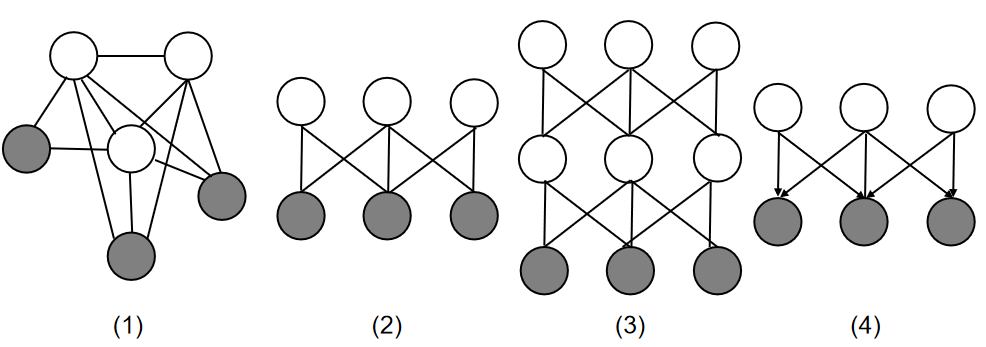
\includegraphics[width=.9\textwidth]{微信图片_20200315123116.png}
    \caption{Boltzmann Machine,Restricted Boltzmann Machine,Deep Boltzmann Machine和Sigmoid Belief Network的概率图模型,灰色的节点代表$v$,白色的节点代表$h$。}
    \label{fig:my_label_1}
\end{figure}
\subsubsection{Boltzmann Machine}
图一中的(1)就是Boltzmann Machine,它的理论依据是很好的,但是并没有很好的办法去解决它。无向图求解概率密度分布,需要转换成最大团势函数的乘积,而Boltzmann Machine中节点之间的关系过于复杂,很难被分解。所以导致计算基本是intractable的。\textbf{无向图的后验不好处理的原因就是连接本身带来相互作用,不容易进行分解,这是无向图模型的硬伤。}
\subsubsection{Restricted Boltzmann Machine}
图一中的(2)就是Restricted Boltzmann Machine,在这个概率图模型中,可以看到,$h$和$v$集合内部的节点都是互相独立的,而集合之间的节点都是相互连接的。结点内部的节点相互独立性可以通过局部马尔可夫性质证明。
\subsubsection{Deep Boltzmann Machine}
图一中的(3)就是Deep Boltzmann Machine,很显然虽然第三层是可观测的,而第一层和第二层节点之间的关系函数很复杂,不可做到相互独立,相互分离,那么同样还是intractable,无法处理。只有当两层是可观测的之后,剩下的那层节点之间才是相互独立的。
\subsubsection{Sigmoid Belief Network}
图一中的(4)就是Sigmoid Belief Network,网络中的概率图模型是有向的,同样$P(h|v)$是求不出来的。根据D-Separation中Head to Head的结构。当中间节点被观测到时,两个head节点是有关系的,不是相互独立的。那么,$h$节点之间就是无法分解的,后验分布求解依然很困难,这就是有向图的explain away问题。

如果,条件分布是Gaussian Distribution就很优美了,根据Gaussian分布的自共轭性,他的条件,联合概率分布都是Gaussian的,这就很好办了,我们之前有用待定系数的方法俩求这个后验概率分布。
\subsubsection{小结}
关于无向图精确推断主要问题就是节点之间的mutual interaction;有向图精确推断主要问题就是explain away。

\section{推断即优化}
\subsection{变分推断}
由于精确推断的难度很高,所以近似推断崛起了。比如EM系列和VI系列。

可以将可观测变量的Log Likelihood转为一个优化ELBO下界和KL散度的形式,从而优化ELBO下界就可以了。Log Likelihood公式表达如下所示:
\begin{equation}
    \frac{1}{N} \sum_{v} \log P(v)
\end{equation}
而$\log P(v)$,可以表达为:
\begin{equation}
    \begin{split}
        \log p(v) = & \log \frac{p(h,v)}{p(h|v)}
        = \log p(h,v) - \log p(h|v) 
        = \log\frac{p(h,v)}{q(h|v)} - \log \frac{p(h|v)}{q(h|v)} \\
    \end{split}
\end{equation}
将等式两边都乘上$q(h|v)$,可以得到:
\begin{equation}
    q(h|v) \log p(v) = q(h|v) \left( \log\frac{p(h,v)}{q(h|v)} - \log \frac{p(h|v)}{q(h|v)} \right)
\end{equation}
因为$q(h|v)$是一个关于$h$的函数,我们将等式两边对$h$积分。其中,左边的$p(v)$和$h$没有关系,而$\int q(h|v) =1$,所以有
$$\int q(h|v) \log p(v) dh = \log p(v) \int q(h|v)  dh = \log p(v) $$
那么有,
\begin{equation}
\begin{split}
    \log p(v) = & \int q(h|v) \left[ \log\frac{p(h,v)}{q(h|v)} - \log \frac{p(h|v)}{q(h|v)} \right]dh \\
    = & \int q(h|v) \left[ \log\frac{p(h,v)}{q(h|v)} \right]dh - \int q(h|v) \left[ \log \frac{p(h|v)}{q(h|v)} \right]dh \\
    = & \int q(h|v) \left[ \log\frac{p(h,v)}{q(h|v)} \right]dh + \int q(h|v) \left[ \log \frac{q(h|v)}{p(h|v)} \right]dh \\
    = & \underbrace{\mathbb{E}_{q(h|v)} \left[ \log\frac{p(h,v)}{q(h|v)} \right]}_{\mathrm{ELBO}} + \mathrm{KL}[q(h|v)||p(h|v)] \\
    \leq & \mathbb{E}_{q(h|v)} \left[ \log\frac{p(h,v)}{q(h|v)}\right]
\end{split}
\end{equation}
因为KL散度是很大于0的,那么我们只要优化ELBO就可以优化$p(v)$了,这就是优化下界的方法。而ELBO可以继续化简为:
\begin{equation}
    \begin{split}
        \mathbb{E}_{q(h|v)} \left[ \log\frac{p(h,v)}{q(h|v)}\right] = & \mathbb{E}_{q(h|v)} \left[ \log p(h,v) - \log q(h|v)\right] \\
        = & \mathbb{E}_{q(h|v)} \left[ \log p(h,v) \right] -\mathbb{E}_{q(h|v)} [ \log q(h|v) ] \\
        = & \mathbb{E}_{q(h|v)} \left[ \log p(h,v) \right] + \mathrm{H}(q(h|v))
    \end{split}
\end{equation}
我们可以将ELBO函数看成$\mathcal{L}(v,h,q)$(q(h|v)是一个函数,函数的函数被称为泛函)。我们的目标就是优化这个函数,从而达到计算$P(v)$。$p(v)$是一个未知的客观真理,所以我们把它当成一个常量来看,而最大化ELBO,实际上也在最小化KL散度。所以,这个算法的目的就是找一个简单的$q(h|v)$去靠近$p(h|v)$,这个$p(h|v)$是不是就是推断。所以说,\textbf{推断即优化}。
\subsection{小结}
本小节主要是通过变分推断的例子来揭示了为什么说推断就是优化,在变分推断的例子中,我用最大化ELBO来使一个简单的分布$q(h|v)$来逼近$p(h|v)$。

\section{总结}
本章,首先介绍了推断的目的是什么,1. 寻找事情发生的原因;2. Learning问题中的使用。然后,分无向图和有向图介绍了精确推断的难点,无向图精确推断主要问题就是节点之间的mutual interaction;有向图精确推断主要问题就是explain away。从而引出了近似推断,然后用变分推断的例子来讲述了推断即优化的思想。整个过程比较流畅。








\end{document}
